\documentclass[article,a4paper]{IEEEtran}
\usepackage{lipsum}
\usepackage[backend=biber]{biblatex}
\usepackage{graphicx}

\addbibresource{refs.bib}
\title{Data formats, databases and clocks in sync, important for IoT}
\author{
\IEEEauthorblockN{Anton Odén}\\
\IEEEauthorblockA{Dept. of Maths and Computer Science\\Karlstad University\\
651 88 KARLSTAD, Sweden}\\
anton.oden@outlook.com
}

\begin{document}

\maketitle

\begin{abstract}
    In IoT systems, efficient data handling is achieved through optimized data formats and scalable storage solutions. Lightweight JSON data exchange, along with reliable clock synchronization protocols, ensures accurate event timing. Moreover, NoSQL databases significantly enhance data retrieval and overall system performance making the most out of resource-constrained environments.
\end{abstract}

\section{Introduction}
The goal of IoT is to give us data to be able to make informed decisions and let us make decisions that would otherwise never been made but because of IoT, is being made and those decisions are contributing to the greater good. In a democratic society in a recurrent event, every citizen with the right to vote is asked to cast a vote on who should make decisions for the next period. The votes are cast in a ballot box and the votes are counted. All the apparatus around the vote and counting it is a costly operation and in Sweden the authorities of election estimated an reelection to cost 200 million Swedish crowns \cite{CostElection}. We do it nevertheless because we believe it is an important decision to be made. Our IoT nodes are also citizens. They are supplying data that could and should help in making informed decisions and just as in politics there is decisions to be made in IoT how close to the end nodes the decision making is to be made. Should all data be communicated to the cloud to be processed there or should the data be processed closer to the end nodes? The answer to that question is not easy and there are many factors to take into consideration. One of the factors is the time it takes to communicate the data to the cloud and back. Another is the bandwidth of the communication channel taken up when all Things communicate on it. The highways has to be broadened to the be able to take the load and there is costs associated with that. 
\newline\newline
This article will walk you through different data formats such as JSON, XML and CSV. It will also briefly touch time and how to synchronize time over the IoT network and finally some database structures where the chooses are many and this article only goes through relational, key-value, document and wide-column databases.  
\section{Data formats}  
The payload needs to be communicated in a data format that both receiver and transmitter knows how to work with. On gateways and servers that has bigger capabilities with memory and compute a complicated data format is no problem. But on small end devices, especially those that run on battery, the data format needs to be lightweight.
\newline\newline      
JavaScript Object Notation (JSON) is THE data format of IoT communication. It doesn't have to be JSON but it has become a standard and is used in many applications and originally known in data transmission between server and client for webpages, hence the JavaScript part and it's an international industry standard (ECMA-404) \cite{JSONstandard}. JSON is lightweight, easy for humans to read, completely language independent and thereby used in many programming languages for data interchange\cite{JSONintro}. JSON makes use of bracket signs to envelope data in objects and can nest data in hierarchies this way. Label and data is separated by a colon and both parts are enveloped by quotation signs. The labeling text could be made as short as one sign and a separate JSON-schema could contain more specified information regarding the data \cite{JSONformat}. The schema is shared between transmitter and receiver and is used for validation of the data in parsing. For minimal bandwidth usage it's a good idea to make labels short and let the commonly known schema act as a translator to make the code more readable.
\begin{figure}
    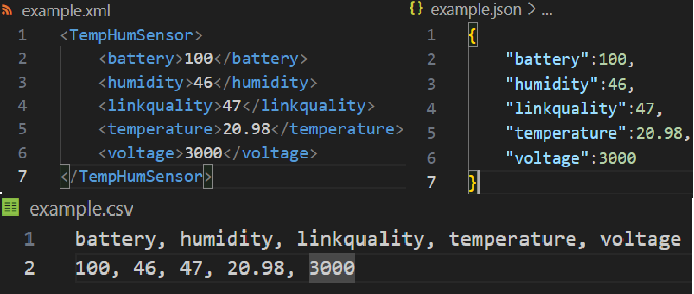
\includegraphics[width=\columnwidth]{JSON-XML-CSV.png} 
    \caption{ Example: XML up-left, JSON up-right, CSV down }
    \label{fig1:XML and JSON example}   
\end{figure}   
\newline\newline
Extensible Markup Language (XML) \cite{XMLdocs} is another common data format for data interchange and is influenced by html in its hierarchical structure where each piece of data (entity) is enclosed within a descriptive tag forming a tree structure that mirrors the relationships between the different entities. As seen in fig1 XML needs opening and closing tags to envelope it's data compared to JSON. It is also dependent on more complex parsing as it allows tags to be given attributes and namespaces to be set to avoid conflicts. This is a problem for IoT devices that needs transmission and processing time to be set to a minimum to not consume battery and it also takes more bandwidth on the network. There are some built in security in XML that does give it some edge in that certain parts of the data could be restricted by further encryption being beneficial in a world of documents \cite{XMLSecurity}. But in IoT where the chunk of data from sensors and actuators is relatively small an encryption on top of all data is probably enough.    
\newline\newline
Comma Separated Value (CSV) \cite{CSVdocs} is a data format that explain itself in its name, every block of data (value) is divided by a comma, as can be seen in fig1. First line in this format optionally contain an header for the data and then each line represent a new set of data. It is a standard since 2005 but originates from before personal computers. The data format is excellent for spreadsheets and the overhead is minimal. A problem thought is that other than headerpart that act as labels, CSV files lack the capability for hierarchy, metadata, datatypes and other structures that JSON and XML has. 
\newline\newline
JSON as we already discussed is the most common used data format in IoT and as could be seen i fig2, the trend overall in all applications is that JSON is taking shares as XML drastically has shrunken in usage since 2004.  
\begin{figure}
    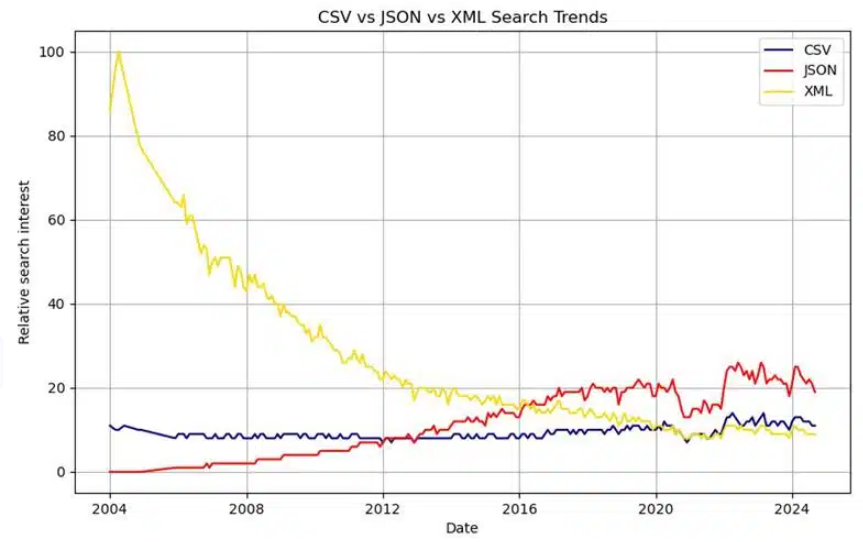
\includegraphics[width=\columnwidth]{DataFormatTrend.png} 
    \caption{ Trend showing rise of JSON compared to XML \cite{CompareJSONXMLCSV} }
    \label{fig2: Trend XML CSV JSON }   
\end{figure}
\section{Clock Synchronization}
A data that is important for most smart decision-making, logging, retrospective analysis etc. is time. Every IoT device has its own idea of the current time and clocks drifts as they are derived from an oscillators frequency. The frequency has manufacturing variability and is influenced by aging, temperature and overdrive so it is difficult for devices to recalculate it's clock by themself. Sensors in IoT in for example a LoRaWAN protocol has the capability to hibernate to conserve battery. To have different knowing of time can do that the server for example thinks a sensor is listening for transmission on a certain time. Thereby a clock synchronization recurrent event is needed for the IoT network (and other networks too).   
\newline\newline 
Network Time Protocol (NTP) \cite{NTPv4} was standardized in 1985 (RFC958) and has now evolved into version 4, published 2010 (RFC5905), being backwards compatible. An NTP network is in hierarchy with the root being stratum 0 that contain a few atomic clocks with super precise time. A few time servers are allowed to communicate with stratum 0 forming stratum 1 and the stratum number increases depending on how many time server jumps the device is from stratum 1. The server or device being closest to stratum 1 in hierarchy and nearest in time from synchronization has the most accurate time. In an IoT network it may be unnecessary for all sensors to have an exact knowledge of the time but what's important is that all the devices within the local network being able to communicate are at synchronization with eachother. 
\newline\newline
The Berkeley algorithm \cite{Berkleyalgo} solves this by assigning one node within the network master status. The masternode is responsible to periodically fetch clock time from all nodes within network. The masternode then calculate an average time between all the nodes, updates its own clock then broadcasts the time over the network for all nodes to update their clocks. Berkley algorithm is a good fit to keep IoT devices within a local network in synchronization and then in wider periods the masternode could fetch timeupdates from closest stratum using NTP to keep the local network relatively synced with global world time.
\begin{figure}
    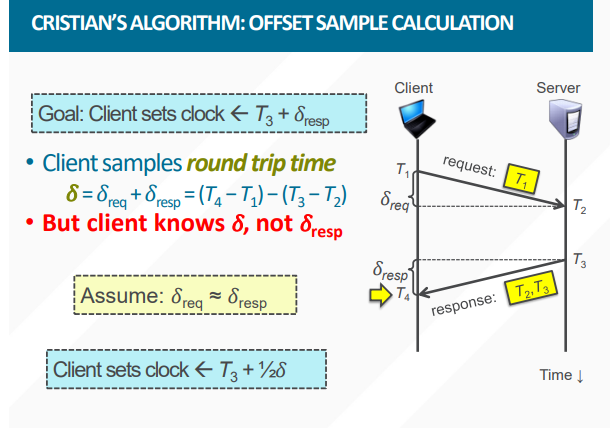
\includegraphics[width=\columnwidth]{Cristianalgo.png} 
    \caption{ Snapshot from slide in \cite{Timesyncslides} }
    \label{fig3: Cristianalgo }   
\end{figure}  
\newline
Latency within the network has been taken into consideration for the masternode in Berkley algorithm to be able to calculate correct average time. This is done via Cristian\'s algorithm as all devices can't be assumed having the same round trip time (RTT). In fig3 client is masternode and server is the nodes that the masternode periodically fetches clock times from \cite{Christianalgo}.  
\section{Data storage}
All data that is being sent needs a space to be stored. Through the network it is stored in fast and small memory close to data processing units deciding where the data is to be stored next. Data is packaged, transmitted, depackaged, processed, packaged, transmitted, depackaged, processed etc. At some point the data stored in a bigger storage called database. Databases have historical been relational databases that are structured similar to spreadsheets. Rows and columns that forms a table. Tables are created with homogeneity in mind such that all the columns in a table exists for the dataset attached to the table. If a dataset exists with labels of data that isn't contained in Table A, a decision has to be made to add a column to the Table A, which would set that column value to null for all other datasets not having that label or creating a new Table B that would contain a lot of similarities with Table A.  
\newline 
Then relationships is built up between tables via unique keys that could in themself be forming another relationship table. Relational databases does give a lot of duplicate spaces for values and many unique keys to keep all relational tables together. It is said that they scale vertically well, meaning a lot of data of the same kind. But lack when it comes to scaling horizontally, meaning adding to much columns to the tables is more stressful for containing order in the structure of a relational database. Relational databases is categories as SQL-databases as SQL (Structured Query Language) is deeply attached to relational databases being the most common language used communicating with an relational database. NoSQL databases is united is that they are non-traditional relation databases. Some categories on NoSQL databases are key-value, document, wide-column \cite{Databasesurvey}, graph and time-series databases.      
\newline\newline
Key-value databases is formed as a long list with keys that each one points to a certain value. Just like a memory registry where every address contain some binary data. In a key-value store the value part is not as in a memory registry restricted to a specific memory size, in a key-value store the value could be anything. Key-value excel when in comes to looking up specific data fast, cause the keys can be in sorted order making binary searching the database possible. Some famous mentioned are Redis and Memcache. 
\newline\newline
Building on top of key-value is another category called document databases that are similar but with availability to search the valuepart. Giving availability to filter and more complex queries to the database. Documents are structured in a XML or JSON manor that makes the transition between storing and transmission of data quick and easy to implement for system development. Some famous document databases is MongoDB and Elasticsearch.
\begin{figure}
    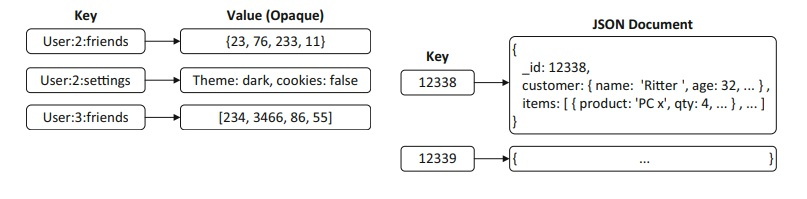
\includegraphics[width=\columnwidth]{keyvaluedocument.jpg} 
    \caption{ Left: Key-value, Right: Document store from \cite{Databasesurvey} }
    \label{fig4: Example Key-value and Document stores }   
\end{figure}  
\newline\newline
Wide-column databases is combining a lot of columns creating a very wide table. The columns are coupled using a rowkey. The rowkey is choosing by the database designer but in an IoT environment with sensors and actuators, including a timestamp in the rowkey could be beneficial. As the rowkey is a value to be searched often, picking an identifier that is often to be contained in a query for filtering would be an good idea. \newline
\begin{figure}
    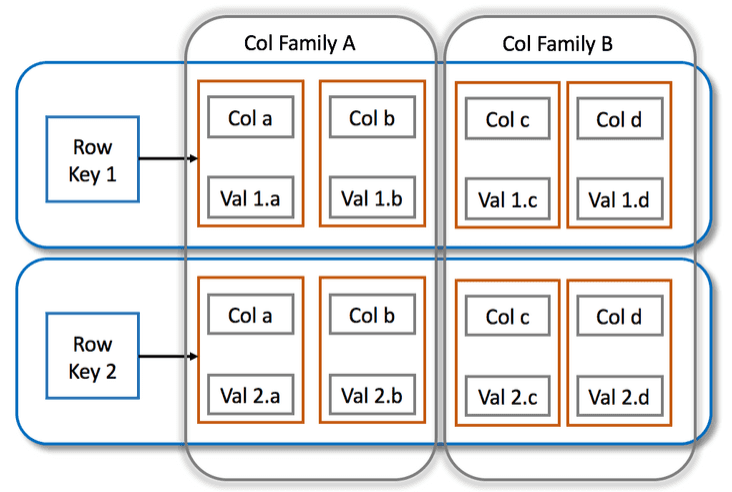
\includegraphics[width=\columnwidth]{widecolumn.png} 
    \caption{ Widecolumn store example from \cite{wide-column} }
    \label{fig5: Example Wide-column stores }   
\end{figure}
For example including device type + timestamp in the rowkey would make is quick to first filter out all temperature-sensors in a wanted period of time. Wide column databases are good for quickly fetching the data from databases that are interesting for the user to know. As a database could hold a lot of columns that is not interesting compared to an relational database that would have to search all columns, even the once we are not interested in. A wide column database after filtering rowkeys only needs to work with the asked for columns. Then if some columns are closely related, the user can decide to group these columns in families. This will ensure in a distributed system, where columns may be stored at different physical places, these grouped columns will with higher potential be groups in the same physical space for quicker retrievals of the total family set. Some famous wide column database structures are Cassandra and HBase.
\section{Conclusion}
Efficient data management is important in IoT systems, ensuring that devices can communicate, synchronize, and store information across networks. Selecting the right data format directly influences the performance of battery-powered IoT devices, with JSON emerging as the dominant choice due to its lightweight and flexible nature. However, alternatives like XML and CSV still serve specific roles based on project needs.
\newline\newline
Clock synchronization plays a critical role in IoT systems, enabling accurate timestamping for event tracking and decision-making. By implementing protocols like NTP and the Berkeley algorithm, IoT networks maintain consistent timing across devices, ensuring reliable communication and data integrity.
\newline\newline
Finally, data storage solutions must support scalable and efficient retrieval methods. While traditional relational databases provide structured organization, NoSQL alternatives—such as key-value, document, and wide-column databases—offer the flexibility needed for handling diverse and evolving datasets. Wide-column databases, in particular, empower IoT applications to efficiently store and retrieve time-series data while minimizing unnecessary computational overhead.
\newline\newline
Hopefully the reader of this article has gotten a better understanding of these subjects as choosing correct tools for data processing will remain vital in building high performance systems.  
\printbibliography

\end{document}